\chapter{Skip Connections}

\section{Residual Units}
为了训练deeper model,并解决梯度消失/爆炸以及网络degradation problem,在ResNets\cite{He2016resnet}中提出,如果在shallower model
中添加identity mapping,那么deeper model理应不会有更高的错误率。
\par
Residual unit表示如下:
\begin{equation}
    \begin{split}
        \mathbf{y}_l &= h(\mathbf{x}_l) + \mathcal{F}(\mathbf{x}_l, \mathcal{W}_l) \\
        \mathbf{x}_{l+1} &= f(\mathbf{y}_l)
    \end{split}
\end{equation}
In ResNet,$h(\mathbf{x}_) = \mathbf{x}_l$ is an identity mapping and $f$ is a ReLU function.
\par
在ResNet中,因为$f$不是identity mapping,所以残差只能ResNet units中学习且信息不能直接传达到后面的层中,
In \cite{He2016identity},希望\textit{propagating information}可以\textit{through theentire network}.
\begin{quotation}
    Our derivations reveal that \textit{if both $h(\mathbf{x}_l)$ and
$f(\mathbf{y}_l)$ are identity mappings}, the signal could be \textit{directly} 
propagated from one unit to any other units, in both forward and backward passes.\cite{He2016identity}
\end{quotation}

if $f$ is also an identity mapping:
\begin{equation}
    \begin{split}
        \mathbf{x}_{l+1} = \mathbf{x}_l + \mathcal{F}(\mathbf{x}_l, \mathbf{W}_l)
    \end{split}
\end{equation}
then we will have:
\begin{equation}
    \begin{split}
        \mathbf{x}_{l+n} &= \mathbf{x}_{l + n - 1} + \mathcal{F}(\mathbf{x}_{l + n -1}, \mathcal{W}_{l + n -1}) \\
        &= \mathbf{x}_{l + n - 2} + \mathcal{F}(\mathbf{x}_{l + n - 2}, \mathcal{W}_{l + n - 2}) + \mathcal{F}(\mathbf{x}_{l + n -1}, \mathcal{W}_{l + n -1})\\
        &= \mathbf{x}_l + \sum_{i=l}^{l+n-1} \mathcal{F}(\mathbf{x}_i, \mathcal{W}_i)
    \end{split}
\end{equation}
相较于plain network(ignoring BN and ReLU is an identity mapping):
\begin{equation}
    \begin{split}
        \mathbf{x}_{l+n} &= \prod_{i=l}^{l+n-1} \mathbf{W}_i \mathbf{x}_i
    \end{split}
\end{equation}
反向传播过程:
\begin{equation}
    \begin{split}
        \frac{\partial \mathcal{E}}{\partial \mathbf{x}_l}
        &= \frac{\partial \mathcal{E}}{\partial \mathbf{x}_{l+n}} \frac{\partial \mathbf{x}_{l+n}}{\partial \mathbf{x}_l} \\
        &= \frac{\partial \mathcal{E}}{\partial \mathbf{x}_{l+n}} \Bigg (1 + \frac{\partial}{\partial \mathbf{x}_{l}}\sum_{i=l}^{l+n-1} \mathcal{F}(\mathbf{x}_i, \mathcal{W}_i)\Bigg)
    \end{split}
\end{equation}
可以看出,上式可以分为两部分,$\frac{\partial \mathcal{E}}{\partial \mathbf{x}_{l+n}}$不经过任何权重信息,可以直接传播到浅层,
只要括号中的第二部分不总是为$-1$,那么\textbf{即使权重任意小也不会发生梯度消失}。

\begin{figure}[H]
    \centering
    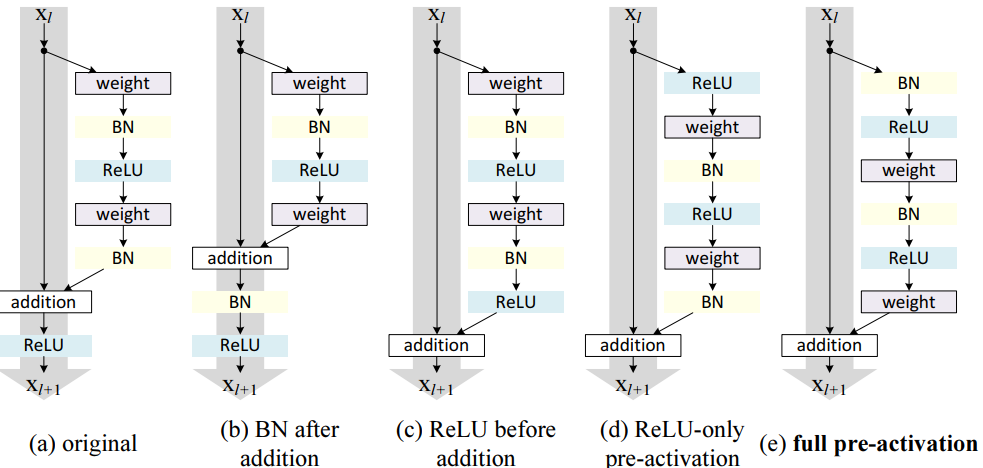
\includegraphics[width=14cm]{images/residual_units.png}
    \caption{Residual Units}
    \label{fig:residual_units}
\end{figure}

以上的分析基于$f$是一个恒等变换,但实际上$f$会影响之前分析的两条信息传播的路径:
\begin{equation}
    \mathbf{x}_{l+1} = f(\mathbf{x}_l) + \mathcal{F}(f(\mathbf{x}_l), \mathcal{W}_l)
\end{equation}
因此,在\cite{He2016identity}提出了新的Residual unit结构pre-activation,等式变为
\begin{equation}
    \mathbf{x}_{l+1} = \mathbf{x}_l + \mathcal{F}(\hat f(\mathbf{x}_l), \mathcal{W}_l)
\end{equation}

\section{The Shattered Gradients Problem}
\begin{quotation}
    A previously unnoticed difficulty with gradients in deep rectifier networks that orthogonal
    to vanishing and exploding gradients. The shattering gradients problem is that, as depth increases,
    \textbf{gradients in standard feedforward networks increasingly resemble white noise}\cite{Balduzzi2017}.
\end{quotation}
\begin{itemize}
    \item Gradients of shallow networks resemble brown noise.
    \item Gradients of deep networks resemble white noise.
    \item Training is difficult when gradients behave like white noise.
    \item Gradients of deep resnets lie in between brown and white noise.
\end{itemize}


\section{恒等映射的意义}
TODO:
\begin{itemize}
    \item 多尺度特征融合
    \item propagating information
\end{itemize}